%--- Load the kaobook class
\documentclass[
    a4paper, % Page size
	fontsize=10pt, % Base font size
	twoside=false, % Use different layouts for even and odd pages (in particular, if twoside=true, the margin column will be always on the outside)
	%open=any, % If twoside=true, uncomment this to force new chapters to start on any page, not only on right (odd) pages
	% secnumdepth=1, % How deep to number headings. Defaults to 1 (sections)
]{kaobook}

\usepackage{subfiles} % Best loaded last in the preamble

% Choose the language
\usepackage[english]{babel} % Load characters and hyphenation
\usepackage[english=british]{csquotes}	% English quotes

\usepackage{mycommands}

\usepackage{preamble}

\usepackage{tikz}

% Load packages for testing
\usepackage{blindtext}
%\usepackage{showframe} % Uncomment to show boxes around the text area, margin, header and footer
%\usepackage{showlabels} % Uncomment to output the content of \label commands to the document where they are used

% Load the bibliography package
\usepackage{kaobiblio}
\addbibresource{minimal.bib} % Bibliography file

% Load mathematical packages for theorems and related environments
\usepackage[framed=true]{kaotheorems}

% Load the package for hyperreferences
\usepackage{kaorefs}

\graphicspath{{images/}{./}{symlinks/illustrations}} % Paths where images are looked for

\makeindex[columns=3, title=Alphabetical Index, intoc] % Make LaTeX produce the files required to compile the index


\begin{document}

%----------------------------------------------------------------------------------------
%	BOOK INFORMATION
%----------------------------------------------------------------------------------------

% \titlehead{Document Template}
\title[Model Correlation in Random Forests]{Model Correlation in Random Forests}
\author[BM]{Benjamin Moser}
\date{\today}
% \publishers{An Awesome Publisher}

%----------------------------------------------------------------------------------------

\frontmatter % Denotes the start of the pre-document content, uses roman numerals

%----------------------------------------------------------------------------------------
%	COPYRIGHT PAGE
%----------------------------------------------------------------------------------------

% \makeatletter
% \uppertitleback{\@titlehead} % Header

% \lowertitleback{
% 	\textbf{Disclaimer} \\
% 	You can edit this page to suit your needs. For instance, here we have a no copyright statement, a colophon and some other information. This page is based on the corresponding page of Ken Arroyo Ohori's thesis, with minimal changes.
	
% 	\medskip
	
% 	\textbf{No copyright} \\
% 	\cczero\ This book is released into the public domain using the CC0 code. To the extent possible under law, I waive all copyright and related or neighbouring rights to this work.
	
% 	To view a copy of the CC0 code, visit: \\\url{http://creativecommons.org/publicdomain/zero/1.0/}
	
% 	\medskip
	
% 	\textbf{Colophon} \\
% 	This document was typeset with the help of \href{https://sourceforge.net/projects/koma-script/}{\KOMAScript} and \href{https://www.latex-project.org/}{\LaTeX} using the \href{https://github.com/fmarotta/kaobook/}{kaobook} class.
	
% 	\medskip
	
% 	\textbf{Publisher} \\
% 	First printed in May 2019 by \@publishers
% }
% \makeatother

%----------------------------------------------------------------------------------------
%	DEDICATION
%----------------------------------------------------------------------------------------

% \dedication{
% 	The harmony of the world is made manifest in Form and Number, and the heart and soul and all the poetry of Natural Philosophy are embodied in the concept of mathematical beauty.\\
% 	\flushright -- D'Arcy Wentworth Thompson
% }

%----------------------------------------------------------------------------------------
%	OUTPUT TITLE PAGE AND PREVIOUS
%----------------------------------------------------------------------------------------

% Note that \maketitle outputs the pages before here
\maketitle



%----------------------------------------------------------------------------------------
%	PREFACE
%----------------------------------------------------------------------------------------

\chapter*{Abstract}

...

%----------------------------------------------------------------------------------------
%	TABLE OF CONTENTS & LIST OF FIGURES/TABLES
%----------------------------------------------------------------------------------------

\begingroup % Local scope for the following commands

% Define the style for the TOC, LOF, and LOT
%\setstretch{1} % Uncomment to modify line spacing in the ToC
%\hypersetup{linkcolor=blue} % Uncomment to set the colour of links in the ToC
\setlength{\textheight}{230\vscale} % Manually adjust the height of the ToC pages

% Turn on compatibility mode for the etoc package
\etocstandarddisplaystyle % "toc display" as if etoc was not loaded
\etocstandardlines % "toc lines as if etoc was not loaded

\tableofcontents % Output the table of contents

% \listoffigures % Output the list of figures

% Comment both of the following lines to have the LOF and the LOT on different pages
\let\cleardoublepage\bigskip
\let\clearpage\bigskip

% \listoftables % Output the list of tables

\endgroup

%----------------------------------------------------------------------------------------
%	MAIN BODY
%----------------------------------------------------------------------------------------

\mainmatter % Denotes the start of the main document content, resets page numbering and uses arabic numbers


%wider contents, more narrow margins
\renewcommand{\marginlayout}{%
 \newgeometry{
	top=27.4mm,
	bottom=27.4mm,
	inner=24.8mm,
	textwidth=127mm, % increased
	marginparsep=5.2mm,
	marginparwidth=39.4mm 
 }%
}
\pagelayout{margin}


\setchapterstyle{plain} % Choose the default chapter heading style
% \pagelayout{wide} % No margins

\chapter{Introduction}

% TODO argue why we are considering the combination of diversity theory and random forests -- in that it is particularly relevant there
% cf also homog ensembles, avg bias equals ens bias? could imply the variance reduction through ens improvement

\section{Overview}

% TODO use the below text as basis?

% Es geht um Ensemble Learning am Beispiel von Random Forests. Das "klassische" Verständnis ist, dass die Kombination von einzelnen Lernern (zB Entscheidungsbäumen) eine niedrigere Varianz (im Sinne von Bias-Variance-Tradeoff) zeigt als der durchschnittliche einzelne Lerner. Weiter hängt das Ausmaß dieser Verbesserung davon ab, wie ähnlich die Vorhersagen der einzelnen Lerner sind. Solche Aussagen wurden allerdings klassischerweise hauptsächlich spezifisch für den Squared-Error-Loss gezeigt. 

% In meiner Arbeit geht es nun zuerst einmal darum, zu verstehen welche Faktoren genau den Fehler eines Ensembles wie beeinflussen. Dazu behandle ich zunächst einmal eine gewisse Theorie (https://arxiv.org/abs/2301.03962), die sich erst in den letzten 1-2 Jahren herausgebildet hat. Das hauptsächliche Ergebnis ist (a) eine allgemeine Bias-Variance-Zerlegung für jeden Loss, (b) eine allgemeine "Ambuigity"-Zerlegung, die die Unterschiede zwischen den einzelnen Lernern berücksichtigt und (c) als Kombination von (a+b) eine eine (exakte) Zerlegung des Ensemble-Fehlers in durschnittlichen Bias der Lerner, durchschnittliche Varianz und ein Maß von *Diversität* zwischen den einzelnen Lernern. 

% Für Bregman Divergences, zu denen u.a. Squared Error und KL-Divergence zählen, vereinfacht sich diese allgemeine Form und es zeigt sich, dass diverse Resultaet, die für spezielle Loss-Funktionen gezeigt wurden, Spezialfälle dieser allgemeinen Struktur sind. Der 0/1-Loss allerdings zählt hier nicht dazu. Hier können wir aber trotzdem noch auf die allgemeine Form der Zerlegung zurückgreifen. 

% Für diese Zerlegungen gebe ich einen alternativen Beweis.

% Ausgehend davon betrachte ich dann Wachstumsstrategien für Ensembles. Eine grundliegende Einsicht ist u.a., dass -- genau wie Bias und Varianz -- die Diversität punktweise gemessen wird ("Erwartungswert über X"). An unterschiedlichen Punkten trägt die Diversität unterschiedlich zum übergreifenden Ensemble-Fehler bei. Insbesondere für Klassifikation unter dem 0/1-Loss ergibt sich hier eine klare binäre Unterscheidung in positiven und negativen Beitrag. Es zeigt sich also, dass Diversität nicht immer vorteilhaft ist, sondern nur an bestimmten Punkten. Dadurch motiviert betrachte ich eine gewisse Wachstumsstrategie, die Diversität an "positiven" Punkten steigert und an "negativen" Punkten verringert. Dies lässt sich wahrscheinlich auch auf das Regressionsproblem übertragen.

% Eine bereits bekannte Wachstumsstrategie für Ensembles von neuronalen Netzen ist "Negative Correlation Learning". Darin wird eben auch Diversität zwischen den einzelnen Lernern erzeugt. Es gab in der Vergangenheit einige Versuche, NCL, ursprünglich für den Squared Error Loss definiert, zu verallgemeinern. Ich argumentiere, dass die obengenannte Zerlegung eine natürliche Verallgemeinerung ist.

\section{Contributions}

% Can motivate many of the choices in decision tree learning from the perspective of bregman divergences

% Alternate proof of the classic bias-variance-decomposition via effect-decompositions and Bregman divergences. This shows that it is but an example for a much broader structure and gives much clearer intuition (instead of just doing the magic in the direct proof).

% Insight that exploiting diversity has to happen through doing so at places where we can \textit{afford} to do so -- i.e. "without affecting bias too much".

% TODO more


\section{Statistics}

We want to reason about algorithms which act on data in a broadly applicable manner. We use statistical language for this. Consider for example a data point $X$ that is used as input for an algorithm. Our intention is to say that this $X$ could be essentially \textit{any} data point from some kind of data source. In other words, we can consider $X$ to be \textit{random}, that is, $X$ is a random variable (a symbol) that can take different values. 
Which values exactly it can take depends on the data source -- the \textit{distribution} of the data. If our data source is a fair $6$-sided die, $X$ can take values in $\Omega = \{ 1, \dots, 6 \}$ and the distribution of values is constant where each outcome has probability $\frac{1}{6}$, i.e. $\prob{}{1} = \dots  = \prob{}{6} = \frac{1}{6}$.
\begin{definition}
  A \textit{probability space} is a triple \((\Omega, \Sigma, \mathbb{P})\)
  where
  \begin{itemize}
  \item \(\Omega\) is an arbitrary set modelling the \textit{sample space}
    i.e.~the set of all possible outcomes.
  \item \(\Sigma\) is a \(\sigma\)-algebra
    over \(\Omega\), modelling the set of \textit{events}.
    % \footnote{A
    %   \(\sigma\)-algebra over \(\Omega\) can be thought of a set of subsets of
    %   \(\Omega\), containing \(\Sigma\), such that it is closed under complement
    %   and countable union and intersection.}
    \item \(\mathbb{P}\) is a function
    \(\Sigma \to [0,1]\) such that \(\mathbb{P}(\Omega)=1\) and
    \(\mathbb{P}\left( \bigcup_{i=1}^\infty A_{i} \right) = \sum_{i=1}^\infty
    \mathbb{P}(A_{i})\) for a countable collection of (pairwise disjoint) sets
    in \(\Sigma\), and models the \textit{probability measure}.
  \end{itemize}
\end{definition}
In the following, we assume an underlying probability space implicitly.
% def random variable
\begin{definition}
  A \textit{random variable} is a quantity
  that depends on a random event, i.e. a function \(\Omega
  \to M\) (commonly, we have \(M=\mathbb{R}\)).
  % that assigns a value to each outcome.
\end{definition}
Further, we not only want to reason about the behaviour of an algorithm with respect to one point $X$ but \textit{many} such points. A basic notion is the \textit{expected value} of $X$. Further, since $X$ is considered random, $f(X)$ is also a random variable and we can talk about the expected value of functions of random variables.
\begin{definition}
  The \textit{probability density function} $f_X$ of a random variable $X$ is a
  nonnegative function such that
  $$
  \mathbb{P}(a < X < b) = \int_a^b f_X(x) dx
  $$
\end{definition} 

\begin{definition}
  The \textit{expected value} (expectation) of random variable \(X\) is
  defined as
  % \[ \mathbb{E}[X] := \int_{-\infty}^\infty x \cdot
  %   \mathbb{P}(X=x) \, dx
  % \]
  
  \[ \mathbb{E}[X] := \int x \cdot
    f_X(x) \, dx
  \]
  where the integral is over the support of $X$. 
\end{definition}

\begin{itemize}
	\item Note that a function \(g(X)\) of a random variable \(X\) is a random variable itself and $\mathbb{E}[g(X)] = {\int g(x)f_X(x) \, dx}$. % law of the unconscious statistician
	\item To emphasize the random
  variable the function is dependent on, we sometimes mention it in the
  subscript and write $\mathbb{E}_X[g(X)]$.
\end{itemize}


\begin{lemma}
  \label{thm:expected-value-properties}
The following facts apply to expected values.
\begin{itemize}
	\item A basic property of expected values is that they are \textit{linear}: For any two random variables $X$, $Y$ and a constant $\alpha$ it holds that $\mathbb{E}\left[ X + Y \right] = \mathbb{E}\left[ X \right] + \mathbb{E}_{}\left[ Y \right]$ and $\mathbb{E}_{}\left[ \alpha X \right] = \alpha \mathbb{E}_{}\left[ X \right]$.
  \item The rule of iterated expectations states that, for any function \(r\):
    \(\mathbb{E}[r(X,Y)] = \mathbb{E}\left[\mathbb{E}[r(X,Y) | X]\right]\) and,
    in particular, \(\mathbb{E}[X] = \mathbb{E}[\mathbb{E}[X|Y]]\)
  \item Jensen's Inequality: Let $X$ be a random variable such that
    $\mathbb{P}(a \leq X \leq b)=1$. If $g: \mathbb{R} \to
    \mathbb{R}$ is convex on $[a, b]$, then
    $
    g(\mathbb{E}\left[ X \right]) \leq \mathbb{E}\left[ g(X) \right]
    $.
  \item If \(X\) and \(Y\) are independent, then \(\mathbb{E}\left[XY\right] =
    \mathbb{E}\left[X\right] \mathbb{E}\left[Y\right]\)
\end{itemize}
\end{lemma}


A random variable is \textit{discrete} if its set of outcomes is a countable set $\{ x_{i}, \dots, x_{n} \}$ with probabilities $\{ p_{i}, \dots, p_{n} \}$. The probability density function then is $f_X(x_i) = \mathbb{P}(X = x_i) = p_i$. The expected value of a discrete random variable is given by a sum.
$$
\mathbb{E}_{}\left[ X \right]  = \sum p_{i} x_{i}
$$

The expected value is a statement depending on the entire distribution. Usually, we do not know the distribution itself, but only have a limited set of samples of it. For instance, we may have a certain number of data points or run an algorithm a certain number of times and observe its output. We can use this set of samples to approximate the value of the expectation. Given that the samples are independent and identically distributed, the arithmetic mean of samples approximates the expected value.
$$
\frac{1}{n} \sum_{i=1}^n x_i ~ \rightarrow ~ \mathbb{E}\left[X\right]  ~ \hspace{1em} \text{as $n \to \infty$}
$$


\section{Supervised Learning}
\label{sec:supervised-learning}

Our goal is to find an algorithm that is able to map objects from $\mathcal{X}$ to outcomes in $\mathcal{Y}$. Objects
are described by their \textit{features}. These are commonly numerical, so $\mathcal{X}$ can be thought of as $\mathbb{R}^d$ where $d$ is the number of features. We will call such a representation of an object an \textit{example}.

In \textit{classification} problems, the outcomes are discrete among $k$ possible outcomes and we refer to them as \textit{labels} or \textit{classes}. For sake of simplicity, we identify these with integers, i.e. $\mathcal{Y}$ can be thought of as the set $\{ 1, \dots, k \}$. In \textit{binary} classification, there are only two possible outcomes. Depending on what is more convenient in the mathematical context, we assume either $\mathcal{Y} = \{0,1\}$ or $\mathcal{Y} = \{-1, 1\}$.
In \textit{regression} problems, the outcomes are continous and we refer to them as \textit{estimates}. We can think of $\mathcal{Y}$ as $\mathbb{R}$.

\begin{marginfigure}
	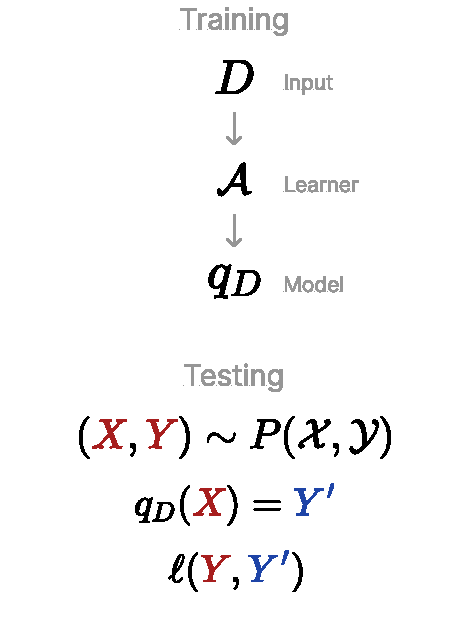
\includegraphics[width=\textwidth]{figma-illustrations/supervised-learning}
	\label{fig:supervised-learning}
	\caption{Illustration of the main components of supervised learning. A learning algorithm $\mathcal{A}$ produces a model $q_D$ given some input $D$. The model is then evaluated on example-outcome pairs of the original data distribution.}
\end{marginfigure}

The desired mapping $q: \mathcal{X} \to \mathcal{Y}$ may be nontrivial such that it is not feasible to come up with explicit rules of how to map examples to outcomes. However, we may try to algorithmically infer such a mapping from a given set of examples and their known outcomes. More specifically, we want to find a deterministic \textit{learning algorithm}, also called \textit{learner}, that, given a random input $D$, produces a mapping $q_D$
\sidenote{
	For the statistical analysis it is essential that the learning algoritm is regarded as deterministic. However, any kind of randomness can be introduced by providing it with random input.
}
.
We call $q_D$ a \textit{model} and note that it is dependent on $D$ .
The task of choosing and configuring a learning algorithm is known as \textit{supervised learning}, which we will be considering herein. 

To analyse the problem, we presuppose a probability distribution $P(\mathcal{X}, \mathcal{Y})$ from which realisations of example-training pairs are drawn. We write this as $(X, Y) \sim P(\mathcal{X}, \mathcal{Y})$ where $(X,Y)$ are random variables from a joint distribution.
This distribution is unknown -- else the problem is trivially solved already. In order for our solution to be widely applicable, we strive to make as few assumptions about $P$ as possible. 

Our given dataset $\{ (\vec{x}_{i}, y_{i}) \}_{i=1}^n$ can be considered a random vector $D$ drawn from $P(\mathcal{X}, \mathcal{Y})^n$ where $n$ is the number of data points
\sidenote{
	The random variable $D$ can actually encompass various sources of randomness. Most prominently, this is the training data. However, it can also reflect inherent randomness in the learning algorithm. For instance, weights in neural networks are sometimes initialised randomly. Unless otherwise stated, this is the intended meaning. If we explicitly distinguish between training data and model parameters, we denote these with the random variable $\Theta$. We explain this formally in \ref{todo}.
	% TODO
}. 
The model $q_D$ produced by our learning algorithm is a function $\mathcal{X} \to \mathcal{Y}$ that depends on the given dataset $D$. The prediction $q_{D}(X)$ is a random variable that depends on the random variables $D$ and $X$.

To be useful, a model should not only accurately estimate outcomes for the given training examples, but also provide reasonable predictions for examples that were not part of the input to the learning algorithm
%
We assess the quality of a single prediction with a \textit{loss function} $\ell: \mathcal{Y} \to \mathcal{Y}$ whose value should be low if the predicted outcome is close to the true outcome. The loss at a single point $x$ with ground-truth value $y$ is then $\ell(y,x)$. 
% To describe the expected loss across the entire distribution, we consider a pair of random variables $(X,Y) \sim P(\mathcal{X}, \mathcal{Y})$. 
%
The \textit{risk} of model $q_{D}$ is the expectation of the loss at a random example-outcome pair.
$$
\text{Risk}(q_{D}) \defeq \mathbb{E}_{(X,Y)\sim P}\left[ \ell(Y, q_{D}(X)) \right] 
$$
%
The quality of a given learning algorithm $\mathcal{A}$ then is the expectation over all possible inputs. This is 
the \textit{expected risk}, also known as \textit{generalisation error}:
$$
\text{GE}(\mathcal{A}) \defeq \mathbb{E}_{D}\left[ \text{Risk}(q_{D}) \right]  = \mathbb{E}_{(X,Y), D}\left[ \ell(Y, q_{D}(X)) \right] 
$$

\section{Bias, Variance and their Effects}
 \label{sec:bias-variance-effects}

Since we are ultimately interested in the generalisation error of an ensemble, the question arises what forces influence it. To this end, one can strive to mathematically express the generalisation error in terms of specific meaningful quantities. A classical decomposition is the \textit{bias-variance-decomposition}. 


\begin{marginfigure} \label{fig:bias-variance-tradeoff}
    \includegraphics[width=\textwidth]{bias-variance/bias_variance_decomposition_with_decision_trees.png}
    \caption{foo!}
    % TODO
\end{marginfigure}

% % TODO bias and variance are measures independent of particular data sample, can use to compare (on same data*set*)

\begin{marginfigure} \label{fig:variance-trees}
    \includegraphics[width=\textwidth]{bias-variance/test_error_of_individual_trees.png}
    \caption{
    Visualising the variance of \textcolor{blue}{Decision Tree} and \textcolor{orange}{Random Forest} models. Each glyph corresponds to the test error of one model trained on a random subset of the full available data. The variation of the test error around the mean test error across many dataset samples is exactly the variance.
    Not only do Random Forests show lower test errors on average, they seem to also have lower variance. We will explain this observation in \ref{todo}
    % TODO because, in fact, ensemble improvement is solely due to reduction in variance
    %   since var(qbar) = mean(var(qi)) - div/div-eff
    % i.e. the difference between mean tree variances and ensemble variance is exactly the ambiguity/diversity-effect
    }
\end{marginfigure}

Informally, the generalisation error can be decomposed as
$$
\text{(error)} = \text{(noise)} + \text{(bias)} + \text{(variance)}
$$
The first quantity, \textit{noise} describes inherent noise in the outcomes. It is intrinsic to the given data and can not be influenced by the choice of learner. The second quantity, \textit{bias} is a measure of precision of the learning algorithm \sidenote{Note that we are measuring the \textit{learning algorithm} and not a produced model.}. Intuitively, it describes how precise, on average, a model typically produced by the learning algorithm is. The third quantity, \textit{variance} describes the spread of the learning algorithm. That is, it describes how different the models produced by the learner will be when given different realisations of the input random variable $D$ -- most prominently, different training data sets. 

This decomposition is an essential tool to understand learning algorithms in general and ensembles such as Random Forests in particular. For the purpose of this thesis, it is important to understand the decomposition and its motivation in detail. 
We will begin by considering the widely known bias-variance-decomposition for regression using the squared-error loss $\ell(y, y') \defeq (y- y')^2$. We will then proceed to generalise the decomposition to arbitrary loss functions.
For sake of clarity, we will from now on take the dependence of $q_{D}(X)$ on $X$ as understood and write only $q_{D}$.

% TODO always hyphen, i.e. "squared-error" loss
The variance of $q_{D}$ with respect to the squared-error loss is commonly defined as the variance of the regressor around its expected value. This is the expected squared error between a random value ($q_{D}$) and the closest non-random value ($\mathbb{E}_{D}\left[q_{D}\right]$). 
$$
\Var{D}{q_{D}} \defeq \mathbb{E}_{_{D}}\left[ (q_{D}- \mathbb{E}_{_{D}}\left[ q_{D} \right] )^2 \right]  = \min_{z} \mathbb{E}_{D}\left[ (q_{D} - z)^2 \right] 
$$
% TODO #todo already use colours here?
As such, $\mathbb{E}_{D}\left[ q_{D} \right]$ is a centroid to the different realisations of $q_{D}$ with respect to the loss function $\ell(y,y') = (y-y')^2$.
This non-random centroid will turn out to be particularly interesting. For a random variable $Z$, let us denote its centroid with respect to $Y$ as
$$
Z^\star \defeq \arg \min_{z} \mathbb{E}_Y\left[ (Y - z)^2 \right]
$$

Let's consider two centroids: One with respect to the label distribution and one with respect to the model outputs.
\begin{itemize}
\item $y^\star(X) = \arg\min_{z} \mathbb{E}_{Y}\left[ (Y - z(X))^2 \right] = \mathbb{E}_{Y|X}\left[ Y \right]$ is the \textit{expected label} % TODO clarify
\item $q^\star(X) = \arg \min_{z} \mathbb{E}_{D}\left[ (q_{D}(X) - z(X))^2 \right]$ is the \textit{expected model}.
\end{itemize}

% As such, for the squared-error loss, we can write
% $$
% \Var{q_{D}} = \mathbb{E}_{D}\left[ L(q_{D}, q^\star) \right] 
% $$
Using this notation, the well-known bias-variance decomposition for the squared-error loss is given as follows.
Note that each variance term is the expected distance in terms of loss to a certain centroid.
\begin{align} \label{thm:sqerr-bias-variance-decomp}
\mathbb{E}_{(X,Y), D}\left[ (Y-q_{D}(X))^2 \right]  
% &= 
%   \mathbb{E}_{(X,Y)}\left[ (Y-y^\star(X))^2 \right]  
% + \mathbb{E}_{X, D}\left[ (y^\star(X) - q_{D}(X))^2 \right]  \\
&= \underbrace{\mathbb{E}_{(X,Y)}\left[ (Y-y^\star(X))^2 \right]   }_{\Var{}{Y} ~~ \text{("noise")}}
+ \underbrace{\mathbb{E}_{X, D}\left[ (q^\star(X) - q_{D}(X))^2 \right]   }_{\Var{}{q} ~~ \text{("learner variance")}}
+ \underbrace{ \mathbb{E}_{X}\left[  (y^\star(X) - q^\star(X))^2\right] 
  }_{\BiasSq{Y, q} ~~ \text{("learner bias")}}
\end{align}
% #todo change BiasSq to just "Bias" -- square is only artifact of squared error
This decomposition is usually derived by expanding the square \cite{todo}. The cross-terms then vanish due to that $  q^\star = \mathbb{E}_{_{D}}\left[ q_{D} \right]$ and $y^\star = \mathbb{E}_{Y|X}\left[ Y \right]$.
This is but a special case of a more general structure applying to a certain class of losses. We will provide a more general proof in lemmas \ref{thm:bregman-collapse-bias} and \ref{thm:bregman-collapse-variances}.

The first term, $\Var{}{Y}$ is independent of $D$ and $q_{D}$. This means we have no means of influencing it with our choice of $q_{D}$.
$\Var{}{Y}$ is also referred to as \textit{noise}, \textit{bayes error} or \textit{irreducible error}. 
The second term, $\Var{}{q}$ measures the variance of our model around its non-random centroid with respect to different realisations of the random training dataset $D$. This can be understood as a measure of spread of the learning algorithm with respect to different realisations of $D$.
The third term, $\BiasSq{q_{D}, Y}$ is the distance in terms of loss between the expected classifier and the expected label. This can be thought of as a measure of precision of our learning algorithm. 

Note that we developed two things:
One the one hand, we derived quantities that measure the notions of bias and variance. On the other hand, by virtue of these quantities appearing in the error decomposition \ref{thm:sqerr-bias-variance-decomp}, we have quantified the \textit{effect} these quantities have on the generalisation error.
This distinction is often overlooked because, like here, for many commonly used losses the quantities and their effects coincide. However, in general this is not necessarily true. We are particularly interested in the \zeroone-loss for classification and a decomposition of it that is independent of the target has been proven to not exist \cite{todo}. We will see that, while we cannot give a bias-variance decomposition for any loss, we can give a more general bias-variance-\textit{effect} decomposition for which the former is a special case.

The variance-effect is the expected change in loss caused by using $q_{D}$ instead of the non-random centroid $q^\star$. Likewise, the bias-effect is the expected change in loss caused by using the expected model instead of the expected label. 
\sidenote{In the original publication \cite{james_GeneralizationsBiasVariance_}, bias-effect is called the \textit{systematic effect}, i.e. the effect of the systematic components. However, it is clearer to call this \textit{bias-effect}, particularly when we begin to introduce notions of diversity in \ref{sec:measures-ensemble-diversity}.}
Formally:
\begin{align*}
\text{Variance-Effect} &\defeq \mathbb{E}_{D,Y}\left[ \ell(Y, q_{D}) - \ell(Y, q^\star) \right] \\
\text{Bias-Effect} &\defeq \mathbb{E}_{D,Y}\left[ \ell(Y, q^\star) - \ell(Y, y^\star) \right] 
\end{align*}

To shorten notation, and to give the equations a shape suggestive for later, we define:
\begin{definition} (Loss-Effect) For a loss functon $\ell$, and random variables $Y, Z, Z'$, we define the change in loss between $Z$ and $Z'$ in relation to $Y$ as:
  $$
  \LE{Z}{Z'} \defeq \ell(Y, Z) - \ell(Y, Z')
  $$
  \label{def:loss-effect}
\end{definition}

Putting this together, we can state a generalised bias-variance decomposition. The classical bias-variance decomposition for squared error (\ref{thm:sqerr-bias-variance-decomp}) is a special case of this (\ref{lemma:the-trick}).

% TODO widepar messes up spacing?
\begin{theorem} (Bias-Variance-Effect-Decomposition \cite{james_GeneralizationsBiasVariance_})
For any loss function $L$, it holds that
% TODO make ystar lowercase in other places aswell (really, it also is a function dependent on x (the bayes classifier?))
% TODO emphasize how this is really about changes in *loss*, directly comparing *predictions* only comes for bregman diverges -- see e.g. arguments on variance reduction
\begin{align*}
\mathbb{E}_{(X,Y), D}\left[ \ell(Y, q_{D}) \right]  
&= 
\underbrace{\mathbb{E}_{Y}\left[ \ell(Y, y^\star) \right]  }_{\text{noise}}
+ \underbrace{\mathbb{E}_{(X,Y)}\left[ \LE{q^\star, y^\star} \right] }_{\text{bias-effect}}
+ \underbrace{\mathbb{E}_{(D,Y)}\left[ \LE{q_D, q^\star} \right] }_{\text{variance-effect}}  \\
\\ 
\text{for} \hspace{1em}
& \LE{q^\star}{y^\star} = \ell(Y, q^\star) - \ell(Y, y^\star) \\ \\
&\LE{q_{D}}{q^\star} = \ell(Y, q_{D}) - \ell(Y, q^\star)
\end{align*}
\end{theorem}
This decomposition holds for \textit{any} loss function $\ell$ since, by linearity of expectation, the individual terms on the right-hand-side simply cancel out. Further, this decomposition is independent of the definitions of $y^\star$ and $q^\star$.


\section{Classifier Margins}

A basic tool in the analysis of classifiers is the notion of margins.  The margin can be thought to represent the classifier's confidence in its prediction. $\prob{}{k|x}$ describes the probability estimated by the classifier that $X$ is of class $k$.

% TODO code snippet illustration plot of margin vector -- should be simple
% TODO disallow page breaks in these boxes
\begin{definition} (Classifier margins \cite{tibshirani_ElementsStatisticalLearning_2017}) The margin for class $k$ of an example $X$ is the difference between the model's confidence that $X$ is of class $k$ and the next-best class:
$$
m(x,y) \defeq \prob{}{y|X} - \max_{j\not=y} \prob{}{j|X}
$$
\begin{itemize}
    \item The vector $m(x) = [m_{1}(x), \dots, m_{K}(x)]^\top$, where $K$ is the total number of classes, is called a \textit{margin vector} iff its components sum to zero. 
    \item For a pair $(X,y)$ of example and true outcome, the model's prediction is correct iff $m_y(X) > 0$ 
\end{itemize}
\label{def:classifier-margin}
\end{definition}
% margin reflects notion of classifier confidence: here, yes, but not necessarily for RF margin

Similarly, we can define a notion of margin for classification ensembles deciding by majority voting. 
% TODO what does "strenght" > 0 mean here? (better than random guessing)

\begin{definition} (Ensemble margins for majority voting \cite{breiman})
The margin for class $y$ of an example $x$ is the difference between the number of member votes for class $Y$ and the number of votes for the next-best class.
	$$
\mr(x,y) \defeq \Mavg \ind{q_{i} = y} - \max_{j \neq y} \Mavg \ind{q_{i} = j}
$$
% TODO maybe express with expectations instead
\label{def:ensemble-margin}
\end{definition}

If ensemble members are parameterised by $\Theta$, from the statistical point of view, we can also write
$$
\mr(x,y) = \prob{\Theta}{q_{\Theta} = y} - \max_{j \not=y} \prob{\Theta}{q=j}
$$
where the probabilities are conditioned on $x$. For binary classification under the \zeroone-loss, the ensemble margin is linearly related to the ratio of incorrect members $\Mavg \Lzo{y}{q_{i}(x)} \approx \prob{\Theta}{q \not= y}$.
$$
\begin{align*}
\mr(x,y) &= \prob{\Theta}{q=y}  - \prob{\Theta}{q \not= y} \\
&= (1 - \prob{\Theta}{q \not= y}) - \prob{\Theta}{q \not= y} \\
&= 1 - 2 \prob{\Theta}{q \not= y}
\end{align*}
$$
So, $\mr(x,y) = 1 - 2 \Mavg\Lzo{y}{q_{i}(x)}$.
% special cases for binary classification, relate to ratio of incorrect members / examples
% TODO -- as such, really close to other decomps

% Let
% $$
% \hat{j} = \hat{j}(\vec{X}, Y) = arg\max_{j\neq Y} \prob{\Theta}{q_{\Theta} = j}
% $$
% denote the next-best vote. So, using the elementary "probability is expectation of indicator" trick:
% \begin{align}
% \mr(\vec{X}, Y)  &= \prob{\theta}{q_{\Theta} = Y} - \prob{\Theta}{q_{\theta} = \hat{j}} \\
% &= \mathbb{E}_{\Theta}\left[ \ind{q_{\Theta} =Y } - \ind{q_{\Theta} = \hat{j}} \right] 
% \end{align}
% Def **Raw margin function** $\rmg(\Theta, \vec{X}, Y)$: Define
% $$
% \rmg(\Theta, \vec{X}, Y) := \ind{q_{\theta} = Y} - \ind{q_{\theta} = \hat{j}}
% $$
% ...such that the RF margin function is the expectation of the raw margin function with respect to $\Theta$:
% $$
% \mr(\vec{X}, Y) = \mathbb{E}_{\Theta}\left[  \rmg(\Theta, \vec{X}, Y)  \right] 
% $$


\section{Bregman Divergences and Centroids}

To measure the difference between predicted and ground-truth outcomes, we use a loss function $\ell$. The choice of loss function depends on the data domain, the learning task and computational considerations. 

Often, learners are analysed with respect to a specific loss, such as the squared-error loss \cite{scornet_ConsistencyRandomForests_2015} for regression or the \zeroone-loss \cite{theisen_WhenAreEnsembles_2023} or the KL-divergence \cite{webb_EnsembleNotEnsemble_2019} for classification. The well-known bias-variance decomposition for the squared-error loss is usually shown directly in teaching materials \cite{tibshirani_ElementsStatisticalLearning_2017, weinberger_Lecture12Bias_}. The question then arises which properties are specific to the loss function and which are part of a more general structure.

We will now define a family of loss functions, called \textit{Bregman divergences}, that encompasses many widely used loss functions in supervised learning (see table \ref{tab:bregman-examples}). 
% We are interested in when and how one can improve the generalisation error by combining multiple models into an ensemble. We will consider generally for arbitrary loss functions, and then identify Bregman divergences of an important special case.

\begin{marginfigure} \label{fig:bias-variance-tradeoff}
    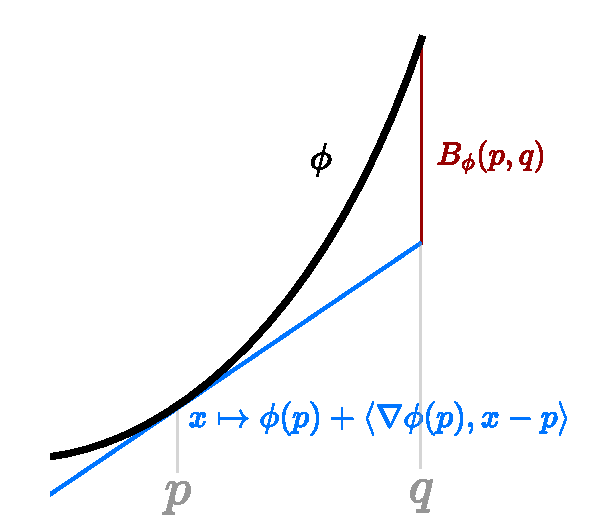
\includegraphics[width=\textwidth]{figma-illustrations/bregman-div-intuition}
    \caption{Given a strictly convex generator $\phi$, the Bregman divergence for points $p, q$ is the difference between the linear approximation around $p$ and $\phi$ at the point $q$. }
\end{marginfigure}
\begin{definition} \label{def:bregman-divergence}
\textit{(Bregman Divergence \cite{todo})} The Bregman divergence $\Breg{p}{q}$  is defined based on a generator function $\phi$ as follows:
$$
\Breg{p}{q} := \phi(\vec{p}) - \phi(\vec{q}) - \inner{\nabla \phi(q)}{(\vec{p} - \vec{q})}
$$
where $\inner{\cdot}{\cdot}$ is the inner product, $\nabla \phi(\vec{q})$ is the gradient vector of $\phi$ at $\vec{q}$ and $\phi: \mathcal{S} \to \mathbb{R}$ is a strictly convex function on a convex set $\mathcal{S} \subseteq \mathbb{R}^k$ such that it is differentiable on the relative interior of $\mathcal{\S{}}$.
\end{definition}


\begin{table*}[hb]
    \centering
    \caption{Examples of commonly used loss functions that are Bregman divergences \cite{clustering with bregman divergences, wood23} }
    % TODO formatting of table
    \begin{tabular}{|l|l|l|l|}
    \hline
        Divergence $\Breg{p}{q}$ & Generator $\phi(q)$ & Domain $S$ & Loss function \\ \hline
        $(p-q)^2$ & $q^2$ & $\mathbb{R}$ & Squared Error \\ \hline
        $x \log \left(\frac{x}{y}\right)+(1-x) \log \left(\frac{1-x}{1-y}\right)$ & $x \log x+(1-x) \log (1-x)$ & $[0,1]$ & Logistic loss \\ \hline
        $\frac{x}{y}-\log \left(\frac{x}{y}\right)-1$ & $-\log x$ & $\mathbb{R}_{>0}$ & Ikura-Saito distance \\ \hline
        $\mid\mid x-y \mid\mid^2$ & $\mid\mid x\mid\mid^2$ & $\mathbb{R}^d$ & Squared Euclidean distance \\ \hline
        $(x-y)^\top A (x-y)$ & $x^\top A y$ & $\mathbb{R}^d$ & Mahalanobis distance \\ \hline
        $\sum_{j=1}^d x_j \log _2\left(\frac{x_j}{y_j}\right)$ & $\sum_{j=1}^d x_j \log _2 x_j$ & $d$-simplex & KL-divergence \\ \hline
        $\sum_{j=1}^d x_j \log \left(\frac{x_j}{y_j}\right)-\sum_{j=1}^d\left(x_j-y_j\right)$ & $\sum_{j=1}^d x_j \log x_j$ & $\mathbb{R}^d_{\geq {0}}$ & Generalized I-divergence \\ \hline
        $\sum_{j=1}^d x_j \log x_j$ & $\sum_{j=1}^d x_j \log x_j$ & $\mathbb{R}_{\geq {0}}$ & Poisson loss \\ \hline
    \end{tabular}
    \label{tab:bregman-examples}
\end{table*}

% \marginfigfromsource{fig:bregman-intuition-1d}{symlinks/illustrations/bregman/bregman-intuition-1d-ikura-saito}

% Recall that in \ref{sec:bias-variance-effects}, we have considered centroids with respect to the squared error, which is symmetric. 
% Bregman divergences are in general not symmetric and hence we need to define \textit{left} and \textit{right} centroids.
% TODO relate centroids to bregman information etc in banerjee_ClusteringBregmanDivergences_2004

\paragraph{Bregman centroids} A common measure is the "statistical" variance $(X - \mathbb{E} \left[ X \right])^2$. One can see that $\mathbb{E}_{}\left[ X \right]$ is in fact the minimizer of the expected squared distances to realisations of $X$:
$$
\mathbb{E}_{}\left[ X \right]  = \arg\min_{z} \mathbb{E}_{X}\left[ (X - z)^2 \right] 
$$
As such, $\mathbb{E}_{}\left[ X \right]$ is a \textit{centroid} of the realisations of $X$ with respect to the squared error. 
This variance of a random variable around its centroid will be a very basic building block in our analysis of the generalisation error of ensembles. Concretely, we will explain that, except for the bias term, the well-known bias-variance decomposition in fact considers only such variances:
\begin{itemize}
\item The variance of the label around the expected label -- this commonly referred to as \textit{label noise} or \textit{irreducible noise}.
\item The variance of a concrete model $q_{D}$ trained on a dataset $D$ around the expected model -- this is commonly referred to as the \textit{(learner) variance}.
\end{itemize}
Further, we will proceed to show that a crucial component to ensemble learning will be the variance of a learner parameterised by $\Theta$ around its expected model with respect to the distribution of $\Theta$.
We will see that all these quantities can indeed be expressed as variances due to a specific property of Bregman divergences. For the \zeroone-loss, this takes a different form.
% TODO somewhere else: this means that bias-variance-covariance decomposition is an artifact of squared error (pullling out the covariance, I think) -- although expressing in terms of disagreement is still possible, cf bounds by theisen.

In order to talk about variances with respect to Bregman divergences, we need a notion of a centroid with respect to a Bregman divergence. Bregman divergences are in general not symmetric and hence there is a \textit{left} and \textit{right} centroid.

\begin{lemma} (Left and right Bregman centroids, \cite{pfau_GeneralizedBiasVarianceDecomposition_})
    Let $B_{\phi}$ be a bregman divergence of generator $\phi: \mathcal{S} \to \mathbb{R}$. For a random variable $Y$ on $\mathcal{S}$, it holds that
\begin{itemize}
    \item the \textit{left Bregman centroid} is $\arg\min_{z}  \mathbb{E}_{z}\left[ \Breg{z}{X}\right] = (\nabla \phi)^{-1} \mathbb{E}_{}\left[ \nabla \phi(X) \right]$
    \item the \textit{right Bregman centroid} is $\arg \min_z \mathbb{E}_{z}\left[ \Breg{X}{z}  \right] = \mathbb{E}_{}\left[ X \right]$
\end{itemize}
\end{lemma}

The left Bregman centroid is the expected value in the dual space implied by $\nabla\phi$. Due to this, we also write 
$$\mathcal{E}\left[X\right] \defeq (\nabla \phi)^{-1}\mathbb{E}_{}\left[ \nabla \phi(X) \right]$$ 
The left Bregman centroid will be important for considering the variance of a learner around its parametrisation $\Theta$.
% TODO a visual here

\paragraph{Generalised variance and Bregman information}

One can define a generalised measure of variance according to a Bregman divergence. As with the case for the squared error, this is the expected distance of a random point to a centroid. 

\begin{definition}
	\label{def:bregman-information}
	The variance around the right Bregman centroid is also known as the 
	\textit{Bregman information} 
  $I_{\phi}(X)$
  \cite{banerjee_ClusteringBregmanDivergences_2004}.
$$
I_{\phi}(X) \defeq \mathbb{E}_{X}\left[ \Breg{X}{\mathbb{E}_X\left[ X \right] } \right] 
$$
\end{definition}
% TODO so decision tree split point search is basically 2-means?!

For example, let $X = \{ X_{1}, \dots, X_{n} \} \subset \mathbb{R}^d$. Then the squared Euclidean distance corresponds to the sample variance \cite{banerjee_ClusteringBregmanDivergences_2004}.
$$
\Breg{p}{q} =~\mid\mid p-q\mid\mid^2 ~ ~ \rightarrow ~ ~ 
I_{\phi}(X) = \frac{1}{n} \sum_{i=1}^n (X_{i} - \mathbb{E}_{}\left[ X \right] )^2
$$
For the KL-divergence, the bregman information is the \textit{mutual information}. Consider a random variable $X$ over probability distributions with probability measure $p$ \cite{banerjee_ClusteringBregmanDivergences_2004}.
$$
\Breg{u}{v} = \sum_{j=1}^d u_{j} \log \left( \frac{u_{j}}{v_{j}} \right) 
~ ~ \rightarrow ~ ~  I_{\phi}(X) = 
\sum_{i=1}^n \sum_{j=1}^m p\left(u_i, v_j\right) \log \frac{p\left(u_i, v_j\right)}{p\left(u_i\right) p\left(v_j\right)}
$$




\chapter{Ensemble Learning}
\label{chapter:ensemble-learning}

\textit{Ensemble Learning} is the method of training $M$ individual models $q_{1}, \dots, q_{M}$ for a given task and aggregating their output by an aggregation function $\bar{q}$ to form an ensemble prediction \cite{zhou_EnsembleMethodsFoundations_2012}. The individual models $q_{1}, \dots, q_{M}$ are referred to as \textit{members}. When all members are constructed using the same learning algorithm, we call it a \textit{homogeneous} ensemble. The learning algorithm is then also referred to as the \textit{base learner}. Otherwise the ensemble is \textit{heterogeneous}. 
When analysing the generalisation error, we refer to $\bar{q}$ as the \textit{ensemble model}. When considering how to actually combine ensemble predictions, we also refer to $\bar{q}$ as the \textit{combiner}. 

\section{Notation}
\label{sec:ensemble-learning-notation}
In the concrete approximation setting, i.e. given an actual ensemble of learners, we consider $\bar{q}$ and $q_{1}, \dots, q_{M}$ to be functions $\mathcal{X} \to \mathcal{Y}$. In the statistical setting, $\bar{q}, q_{1}, \dots, q_{M}$ are random variables dependent on a random variable $X$ that represents the query example. Further, combiner and members depend on the input $D$ to the ensemble construction algorithm. For sake of brevity, this dependence is implicit in the notation and we write $q_{i} \defeq q_{i}(X;D)$.

In the original supervised learning setup (see section \ref{sec:supervised-learning}), we considered $D$ to be input to the learning algorithm, particularly including any training data or randomness. Now we are considering multiple learning algorithms. Each of these individual learners receives its own input. For instance, each learner may be trained on a random subset of the available training data (this is \textit{bootstrapping}, see section \ref{sec:bootstrapping}). To this end, we consider $D$ to be a random vector of random variables $(D_{i}, \dots, D_{M})$. 
Due to the law of total expectation, one can write
$$
\mathbb{E}_{D}\left[ \ell(y, q(x; D_{i})) \right]  = \mathbb{E}_{D_{i}}\left[ \ell(y, q(x; D_{i})) \right] 
$$
even if there are dependencies between the components of $D$. This means that for an individual member $q_{i}$, an expectation over $D$ reduces to an expectation over $D_{i}$. This justifies considering expectations over $D$ in general.
In some cases, it is clearer to distinguish between input training data and other random parametrisation of the individual learner. In this case, we take $D$ to be the training data and $\Theta$ to be a random variable representing other parameters. One can then write $\bar{q} = \mathbb{E}\left[q(x; \Theta)\right]$.


% Ultimately, we are interested in the generalisation error of the ensemble given by $\mathbb{E}_{(X,Y),D}\left[ \ell(Y, \bar{q}_{D}(X)) \right]$ where the subscript indicates that the ensemble model depends on the random variable $D$. Since $\bar{q}$ is produced by aggregating the member outputs $q_{1}, \dots, q_{M}$ the essential question is how the member models have to behave in order for ensemble techniques to be effective. 

\section{Methods}
\label{sec:ensemble-learning-methods}
There are three main variants of ensemble learning \cite{mienye_SurveyEnsembleLearning_2022}:
\begin{itemize}
\item \textit{Parallel}: All members are trained independently. The outputs of all members are then aggregated to form the ensemble prediction.
\item \textit{Stacking} or \textit{Meta-Learning}: All members are trained independently. The member outputs serve as input data for another learning algorithm, which then provides the ensemble prediction.
\item \textit{Sequential}: Members are trained in sequence. The output of the previous ensemble member informs the construction of the next member.
\end{itemize}
% TODO diagrams
Random Forests \cite{breiman_RandomForests_2001} are an example of parallel ensemble construction. $M$ decision trees are constructed independently and the tree's predictions are aggregated by a kind of mean (see section \ref{sec:decision-trees}). A classical example for sequential ensemble construction is \textit{Boosting} \cite{schapire_BoostingFoundationsAlgorithms_2012}. In boosting algorithms, the ensemble combiner $\bar{q}$ is not a mean but a (weighted) sum $\bar{q} = \sum_{i=1}^M \alpha_{i}q_{i}$. The first member $q_{1}$ provides a base prediction. Successive members are then trained to predict not an output value but \textit{increments} (\textit{pseudo-targets}) to the base prediction such that the sum $\alpha_{1}q_{1} + \alpha_{2}q_{2} + \dots$ moves towards a more precise prediction. 
In this thesis, we will focus on the Random Forest learner and variations of it. Although it can be seen as a parallel ensemble construction method, we will see that the distinction between parallel and sequential approaches blurs (see \ref{todo}).

\section{Motivation}
\label{sec:ensemble-learning-motivation}

We will now review some arguments that motivate ensemble learning. We do this to provide context to the results in section \ref{later}, which also clearly show when and how ensemble learning is beneficial.


The arithmetic mean combiner can be seen as approximating an expectation over member models, i.e. $\bar{q} = \mathbb{E}_{\Theta} \left[q_{\Theta}\right]$.
This motivated \citeauthoryear{abe} to invoke Jensen's inequality
\marginnote{Jensen's inequality, in a probabilistic setting, states that, for a function $\phi:\mathbb{R} \to \mathbb{R}$ and a random variable $X$
$$
\phi \text{~convex} \rightarrow \phi\left(\mathbb{E}_{}\left[ X \right] \right) \leq \mathbb{E}_{}\left[ \phi(X) \right] 
$$
}
. For a loss function $\ell$ that is convex in its first argument, it holds that
$$
\underbrace{
\ell(\mathbb{E}_{\Theta}\left[ q_{\Theta}(X)\right] , Y  ) 
}_{\text{"ensemble loss"}}
~ ~ \leq ~ ~ 
\mathbb{E}_{\Theta}\left[ 
\underbrace{
\ell(q_{\Theta}(X), Y)  
}_{\text{"member loss"}}
\right]
$$
and thus
$$
\mathbb{E}_{{\Theta}}\left[ \ell (q_{\Theta}(X),Y) \right]  -
\ell(\mathbb{E}_{\Theta}\left[ q_{\Theta}(X) \right] ,Y ) \geq 0
$$
This shows that, for convex loss functions and the arithmetic mean combiner, the ensemble loss is always smaller-equal than the average member error.
\citeauthoryear{abe} interpret this \textit{Jensen gap}, i.e. the difference between these quantities, as a measure of ensemble improvement. 

% TODO would probably also be nice to put Jensen argument here

\paragraph{Variance reduction for squared-error regression} 
A common motivation for using ensembles over single models is that the combination of models reduces the variance as compared to the expected variance of a single model. Further, the bias is not affected, i.e. the ensemble bias is the same as the bias of any member.
In the regression setting, under the squared-error loss and the arithmetic mean combiner%
% \sidenote{
% 	As we will see in \ref{section:div}, the choice of loss function actually determines the definition of combiner $\bar{q}$.
% }
, this can be seen as follows~\cite{stackexchange}. Assume $q_{1}, \dots, q_{M}$ are identically and independently distributed with equal variance $\sigma^2$.
$$
	\Var{}{\bar{q}} = \Var{}{\Mavg q_{i}} = \frac{1}{M^2} \sum_{i=1}^M \Var{}{q_{i}} = \frac{1}{M} \sigma^2
$$
As the number of members $M$ increases, the ensemble variance is reduced. Further, one can also see that the interactions between members determine the variance reduction. Assume ensemble members have equal pairwise covariance. Then 
$$
\rho \defeq \frac{\text{Cov}(q_{i}, q_{j})}{\sigma^2} ~ ~ \leftrightarrow \text{Cov}(q_{i}, q_{j}) = \rho \sigma^2
$$
Further, 
$$
\Var{}{\bar{q}} = \Var{}{\Mavg q_{i}} = \frac{1}{M^2} \left( 
\underbrace{
\sum_{i=1}^M \Var{}{q_{i}}
}_{M\sigma^2}
+
\underbrace{
2 \sum_{i<j}^M \text{Cov}(q_{i}, q_{j})
}_{M(M-1)\rho \sigma^2}
\right)
= \frac{\sigma^2}{M} + \frac{M-1}{M} \rho \sigma^2
$$
One can show that $\rho \geq 0$ \cite{louppe_UnderstandingRandomForests_2015}. This illustrates that ensemble variance is smallest if the members are not correlated, i.e. $\rho \approx 0$. 

\paragraph{Variance reduction for classification margins} For classification, a classical analysis is the bound given by \citeauthor{breiman_RandomForests_2001} in \cite{breiman_RandomForests_2001}, in which Random Forests are first introduced. The basic idea is to consider variances with respect to the ensemble margin margin (see def. \ref{def:ensemble-margin}).
% TODO recap in margin
% TODO need to define notion of "margin" for RFs
% TODO definition of error in terms of margins > 0
We open with Chebychev's inequality to bound the generalisation error in terms of the variance of the ensemble margin.
% TODO this mg > 0 is for 0/1-loss, right?
$$
\mathbb{E}\left[ \ell(Y, \bar{q}(X)) \right]  = \prob{}{\mr(X, Y; D) < 0 }  ~ ~ \leq ~ ~ \frac{\Var{}{\mr(X, Y; D)  }}{\mathbb{E}_{X,Y}\left[ \mr(X, Y; D)  \right]^2}
$$
We can already see that we have an interaction between the performance of the individual members, as reflected in the ensemble margin $\mathbb{E}_{X,Y}\left[ \mr(X, Y; D)  \right]$ and what we will shortly show to be indicative of the diversity of the ensemble. The generalisation error is in part determined by the ratio of these two quantities.

$s \defeq \mathbb{E}_{X,Y}\left[ \mr(X, Y; D)  \right]$ is also called the \textit{strength} of the ensemble.
$s$ is assumed to be non-negative. For binary classification, this is equivalent 
% TODO make sure
to the weak-learner assumption (see \ref{def:weak-learner}).

Note that
$$
\mr(X, Y;D) = \mathbb{E}_{\Theta}\left[ 
\underbrace{
\ind{q_{i}=Y} - \ind{q_{i}=K} 
}_{
\defeq ~\rmg(X, Y, \Theta) 
}
~|~(X,Y), D \right] 
$$
where $K$ is the next-best class and we define the \textit{raw margin function} $\rmg(X, Y, \Theta)$ to be the inner part of that expectation. So, 
$\mr(X, Y;D) = \mathbb{E}_{\Theta}\left[ 
\rmg(X, Y, \Theta) 
~|~(X,Y), D \right]$. Notably, $\mr$ is the \textit{ensemble} margin measuring the ratio of incorrect members and $\rmg$ corresponds to the \textit{classifier} margin, measuring the ratio of incorrectly classfied examples by a member.

\begin{theorem} (\cite{breiman_RandomForests_2001})
The variance of the ensemble margin can be expressed in terms of the covariance between the raw member margins of two members parameterised by \textit{i.i.d} $\Theta, \Theta'$.
	$$
	\Var{X,Y}{\mr(X,Y;D)} = \mathbb{E}_{\Theta, \Theta'}\left[ \text{Cov}_{(X,Y)}(\rmg(\Theta), \rmg(\Theta') ) \right] 
	$$
\end{theorem}
\begin{proof}
	% TODO for coolness, some margin notes here that contain the definitions used in the steps (def of variance, law of total exp etc) -- also to show that we didnt just mindlessly copy this btu actually worked through it
	For brevity, we write
	  $Z \defeq (X,Y)$,
	 $\mr(Z) \defeq \mr(X,Y;D)$ and
	 $\rmg(\Theta) \defeq \rmg(X,Y;\Theta)$.
By the definition of variance, have
\begin{align*}
\Var{Z}{\mr(Z)} &= \mathbb{E}_{Z}\left[ \left(\mr(Z) - \mathbb{E}_{Z}\left[ \mr(Z) \right]\right) ^2 \right]  \\
&= \mathbb{E}_{Z}\left[ \mr(Z)^2 \right] - \mathbb{E}_{Z}\left[ \mr(Z) \right] ^2 \\
\end{align*}

For the left term, by the rule of iterated expectation and the fact that $Z$ and $\Theta$ are independent (see lemma \ref{thm:expected-value-properties}), it holds that
$$
\mathbb{E}_{Z}\left[ \mr(Z) ^2 \right]  = \mathbb{E}_{Z}\left[ \mathbb{E}_{\Theta}\left[ \rmg(\Theta) \mid Z \right] ^2  \right] = \mathbb{E}_{Z, \Theta}\left[ \rmg(\Theta)^2 \right] % by law of total \exp ectation
= \mathbb{E}_{\Theta}\left[ \mathbb{E}_{Z}\left[ \rmg(\Theta) ^2 \right]  \right] 
$$
% or alternatively (by "property")
% $$
% \mr(Z)^2 = \mathbb{E}_{\Theta, \Theta'}\left[ \rmg(\Theta) \rmg(\Theta')  \right] 
% $$
% so 
% $$
% \begin{align}
% \mathbb{E}_{Z}\left[ \mr(Z) ^2 \right] = \mathbb{E}_{Z}\left[ \mathbb{E}_{\Theta, \Theta'}\left[ \rmg(\Theta) \rmg(\Theta')  \right]  \right]  &= \mathbb{E}_{Z}\left[ \mathbb{E}_{\Theta}\left[ \rmg(\Theta)  \right]^2  \right]  = \mathbb{E}_{Z, \Theta}\left[ \rmg(\Theta) ^2 \right] \\ \\
% &= \mathbb{E}_{\Theta, \Theta'}\left[ \mathbb{E}_{Z}\left[ \rmg(\Theta) \rmg(\Theta') \right]  \right]  \\
% &= \mathbb{E}_{\Theta}\left[ \mathbb{E}_{Z}\left[ \rmg(\Theta) ^2 \right]  \right] & (l)
% \end{align}
% $$

For the right-hand-side term, we can make use of the fact that, for a function $f$, it holds that $\mathbb{E}_{\Theta}\left[ f(\Theta)^2 \right] = \mathbb{E}_{\Theta, \Theta'}\left[ f(\Theta) f(\Theta') \right]$ where $\Theta$ and $\Theta'$ are independent and identically distributed. Then we apply the rule of iterated expectation and exploit that $Z$ and $\Theta$ are independent.
\begin{align*}
\mathbb{E}_{Z}\left[ \mr(Z) \right] ^2 &= \mathbb{E}_{Z}\left[ \mathbb{E}_{\Theta}\left[ \rmg(\Theta) \mid Z \right] \cdot \mathbb{E}_{\Theta'}\left[ \rmg(\Theta') \mid Z  \right]  \right] % by lemma   \\ \\ \\
\\ 
&=  \mathbb{E}_{Z}\left[ \mathbb{E}_{\Theta}\left[ \rmg(\Theta) \right] \mathbb{E}_{\Theta'}\left[  \rmg(\Theta') \right]  \right]   \\
&= \mathbb{E}_{\Theta, \Theta'}\left[ \mathbb{E}_{Z}\left[ \rmg(\Theta) \right] \mathbb{E}_{Z}\left[ \rmg(\Theta') \right]    \right] \\
&= \mathbb{E}_{\Theta}\left[ \mathbb{E}_{Z}\left[ \rmg(\Theta)   \right]^2  \right]
% \\ \\
% &= \mathbb{E}_{Z}\left[ \mathbb{E}_{\Theta, \Theta'}\left[ \rmg(\Theta) \rmg(\Theta') \mid Z  \right]  \right] % law of it \exp
% \\ \\
% &= \mathbb{E}_{Z, \Theta, \Theta'}\left[ \rmg(\Theta) \rmg(\Theta') \right]  \\ \\ 
% &= \mathbb{E}_{\Theta, \Theta'}\left[ \mathbb{E}_{Z}\left[ \rmg(\Theta) \rmg(\Theta') \right]  \right]  \\ \\
% &= \mathbb{E}_{\Theta}\left[ \mathbb{E}_{Z}\left[ \rmg(\Theta)^2 \right]  \right] \\ \\ \\ 
% &= \mathbb{E}_{Z}\left[ \mathbb{E}_{\Theta}\left[ \rmg(\Theta) \mid Z \right] ^2 \right]  \\
% &= \mathbb{E}_{Z, \Theta}\left[ \rmg(\Theta)  \right]^2 & by lemma \\
% &= \mathbb{E}_{\Theta, \Theta'}\left[ \mathbb{E}_{Z}\left[ \rmg(\Theta) \rmg(\Theta') \right] ^2  \right] 
\end{align*} 
Plugging these equalities in the decomposition of variance above proves the statement.
\begin{align*}
\Var{Z}{\mr(Z) } &= \mathbb{E}_{\Theta}\left[ \mathbb{E}_{Z}\left[ \rmg(\Theta) ^2 \right]   \right]  - \mathbb{E}_{\Theta}\left[ \mathbb{E}_{Z}\left[ \rmg(\Theta)  \right]^2  \right]  \\
&= \mathbb{E}_{\Theta}\left[ \mathbb{E}_{Z}\left[ \rmg(\Theta) ^2 \right] - \mathbb{E}_{Z}\left[ \rmg(\Theta)   \right]^2   \right]  \\
&= \mathbb{E}_{\Theta}\left[ \Var{Z}{\rmg(\Theta)} \right]  \\
&= \mathbb{E}_{\Theta, \Theta'}\left[ \text{Cov}_{Z}(\rmg(\Theta), \rmg(\Theta') ) \right] 
\end{align*}
% TODO indicate RV D, missing here
% TODO re-derive a similar upper bound starting from ambiguity decomp and apply triangle ineq for 0-1-loss
\end{proof}



% By the moment definition of variance, it holds that

% $$
% \Var{\mr(X, Y; D) } = 
% \mathbb{E}\left[ \mr(X, Y; D)^2 \right] 
% - \left( \mathbb{E}\left[ \mr(X, Y; D)  \right]   \right)^2
% $$
% For the first term, by definition of $\rmg(X, Y; \Theta)$, we have
% $$
% \mathbb{E}_{}\left[ \mr(X, Y; D) ^2 \right]  = \mathbb{E}_{D(X,Y)}\left[ \mathbb{E}_{\Theta}\left[ \rmg(X, Y; \Theta) ~|~(X,Y), D \right]^2  \right] 
% $$
% For sake of brevity, we write $\text{rmg}(\Theta) \defeq \rmg(X, Y; \Theta)$. Further, for the right-hand-side term, since members are identically independently distributed, 
% \begin{widepar}
% \begin{align}
% \mathbb{E}_{}\left[ \mr(X, Y; D) ^2 \right] &= \mathbb{E}_{D, (X,Y)}\left[  ~ ~ 
% \mathbb{E}_{\Theta}\left[ \text{rmg}(\Theta) \mid (X,Y),D \right]    ~\cdot~
% \mathbb{E}_{\Theta'}\left[ \text{rmg}(\Theta') \mid (X,Y),D \right] 
% ~ ~ \right] \\
% &= \mathbb{E}_{\Theta, \Theta', D}\left[ \mathbb{E}_{(X,Y)}\left[ \text{rmg}(\Theta) \cdot \text{rmg}(\Theta')  \right]  \right]  \\
% &= \mathbb{E}_{\Theta, \Theta', D}\left[ \text{Cov}(\text{rmg}(\Theta), \text{rmg}(\Theta') ) + \mathbb{E}_{(X,Y)}\left[ \text{rmg}(\Theta) \right]  \cdot \mathbb{E}_{(X,Y)}\left[ \text{rmg}(\Theta')  \right]  \right] 
% \end{align}
% \end{widepar}
% Combining these results for the left- and right-hand-side term, one can show that
% $$
% \Var{\mr(X, Y; D) } =
% \Var{\mathbb{E}_{(X,Y)}\left[ \mr(X, Y; D)  \right] } + 
% \mathbb{E}_{\Theta, \Theta', D}\left[ \text{Cov}(\text{rmg}(\Theta), \text{rmg}(\Theta')   ) \right] 
% $$
% TODO first variance is over D
% TODO check whether that is actually similar to BVCov decomp once we've written that.  Maybe the variance here is over sth else
% Still, the upper bound is illustrative. The variance term is the variance over all datasets $D$ of the expected margin. This variance is supposedly small since ...
% TODO https://towardsdatascience.com/the-statistics-behind-random-forests-2bfe2e8116f9

This
% TODO better ref an eq
is the expected covariance between the classification margins of two individual members. As we have seen before for the regression case, the generalisation error is lower if individual members are uncorrelated. Unfortunately, this is only an upper bound. In section \ref{sec:bias-variance-covariance}, we will be able to make the same observation from an exact decomposition of the generalisation error.


\paragraph{Ensemble bias equals average member bias}
It can be shown that the bias of a homogeneous ensemble with the arithmetic mean combiner is equal to the average bias of the ensemble members \cite{louppe_UnderstandingRandomForests_2015}. We will give an illustrative argument for the arithmetic mean combiner here.
We will show this in detail in a more general and inuitive way in section \ref{todo}.

Consider individual learner inputs $D = (D_{1}, \dots, D_{M})$. Each member depends on some $D_{i}$ and the combiner $\bar{q}$ depends wholly on $D$. Assuming that $D_{1}, \dots, D_{M}$ are independent and identically distributed, we can write

$$
\mathbb{E}_{D, \Theta}\left[ \bar{q} \right] = \mathbb{E}_{D}\left[ \Mavg q_{D_{i}} \right] = \Mavg \mathbb{E}_{D_{i}}\left[ q_{D_{i}} \right] = \mathbb{E}_{D'}\left[ q_{D'} \right]
$$
where $D'$ is distributed as any $D_{i}$. We can conclude $\mathbb{E}_{D}\left[ \bar{q} \right] = \mathbb{E}_{D}\left[ q_{D} \right]$ (see section \ref{sec:ensemble-learning-notation}).
This implies
% TODO pull this out into lemma, also using this somewhere else
% need to reorder a bit anyway, havent even introduced star notation yet
$$
\bar{q}^\star = \mathbb{E}_{D}\left[ \bar{q} \right]  = \mathbb{E}_{D}\left[ q_{D} \right]  = q^\star
$$
and thus the bias of the ensemble is the same as the bias of a member model $q$:
$$
\mathbb{E}_{X}\left[ \ell(y^\star(X), \bar{q}^\star(X)) \right] 
= \mathbb{E}_{X}\left[ \ell(y^\star(X), q^\star(X)) \right] 
$$
This argument depends on the linearity of expectations, the arithmetic mean combiner and the fact that the ensemble members are constructed following the same parameter distribution. In other words, the ensemble is \textit{homogeneous}. We will later show this more directly for any loss function and any combiner (see \ref{sec:unchanged-bias}).

This implies that the ensemble improvement for homogeneous ensembles under the arithmetic mean combiner is solely due to variance reduction.

\section{Bias, Variance and Covariance}
\label{sec:bias-variance-covariance}

In section \ref{sec:ensemble-learning-motivation}, we have already seen hints that the covariance between members is an essential factor to ensemble performance. Indeed, the notion of covariance and uncorrelatedness has been a guiding thought in the literature \cite{didaci_DiversityClassifierEnsembles_2013, brown_ManagingDiversityRegression_2005, buschjager_GeneralizedNegativeCorrelation_2020}.
We will now introduce an exact decomposition of the ensemble error for the squared-error loss that includes the average covariance between member predictions.
\begin{theorem} (Bias-Variance-Covariance decomposition \ref{ueda, brownManaging})
It holds that
$$
\begin{align}
\mathbb{E}_{(X,Y),D}\left[ (y - \bar{q})^2 \right]  &= \overtext{bias}^2 + \frac{1}{M} \overtext{var} + \left( 1 - \frac{1}{M} \right) \overtext{covar} \\ \\ 
\text{for} ~ ~ & \overtext{bias} =_{\text{def}} \Mavg (\mathbb{E}_{D}\left[ q_{i}  \right] - y) \\
& \overtext{var} =_{\text{def}} \Mavg \mathbb{E}_{D}\left[ (q_{i} - \mathbb{E}_{D}\left[ q_{i} \right])^2  \right]  \\
& \overtext{covar} =_{\text{def}} \frac{1}{M(M-1)} \sum_{i \not= j} \mathbb{E}_{D}\left[ (q_{i} - \mathbb{E}_{D}\left[ q_{i} \right] ) (q_{j} - \mathbb{E}_{D}\left[ q_{j} \right] ) \right] 
\end{align}
$$
\end{theorem}
This can be interpreted as a decomposition into characteristics of individual learners (mean bias and variance), plus a quantity describing the interactions between diferent learners. Again, one can see that ensemble performance profits if members are uncorrelated.
However, this decomposition is only given for the squared error and the arithmetic mean combiner. 

\section{Applications}
...

\chapter{Random Forests}
\subfile{chapters/random-forests.tex}

\chapter{Diversity}

\subfile{chapters/bias-variance-effects.tex.md}

\subfile{chapters/diversity-diversity-effect.tex.md}


% TODO is derivation of breiman bound similar to rationale of covariance decomp?

\section{Ensemble Improvement}
\subfile{chapters/ensemble-improvement.tex}

\chapter{Growth Strategies}

Some general intuition on the idea behind encouraging diversity (always tradeoff with avg member error)

\section{Review} 
Maybe here also review on existing methods, or otherwise relate and motivate where needed.


\section{Binary classification and Dynamic Random Forests}
\subfile{chapters/dynamic-random-forests.tex}

\subsection{"Boosting" rationale for example weighting in classifier ensembles}

re. spike: not super surprising, if there are only 1, 2, 3 trees, weights as ratio of incorrect trees are super extreme -- motivation to dampen

would be good to put here to explain "spike". Can such a spike be observed in boosting methods?

initial increase in bias also observed for classical boosting models? (wood23 p26)

% TODO weighted bootstrapping actually *too* extreme? all happens in first handful of trees. super hard increase in bias. might be better if slower. (cf learning rate for boosting)
% can (probably) dampen weights by inputting them to a linear function (see sketch)


\subsection{Outlook: Generalising to other losses}

We can reach a similar insight for the general case of any loss function.
% TODO wording. doesnt flow anymore. similar to what?
% , although the theoretical analysis is more involved here since under continous loss functions, the effect of the precision of the ensemble and member predictions are continous aswell.
For Bregman divergences, the main difference is that the ensemble improvement / ambiguity-effect
% TODO resolve double terms
is always non-negative. By the ambiguity decomposition \ref{ambig-decomp} we can see that the ensemble error is always expressed by the gap between average member error and average ambiguity. 
$$
\Breg{y}{\bar{q}} = \Mavg \Breg{y}{q_{i}} - \Breg{\bar{q}}{q_{i}} \geq 0
$$
As such, there are no points with "bad diversity", which contribute negatively to the ambiguity(-effect) term, as is the case for the \zeroone-loss (\ref{prev-section}).

However, we may still consider the above equation and how choosing the next member $q_{M+1}$ affects it. Suppose the average member loss $\Mavg \Breg{y}{q_{i}}$ is large. Then this is either mitigated by the diversity $\Mavg \Breg{\bar{q}}{q_{i}}$, in which case the ensemble error is still low; or it is not, in which case the ensemble error too is large. 
However, if the average member loss $\Mavg\Breg{y}{q_i}$ itself is small, there cannot be much diversity since, it is bounded by the average member error.  Because of this, we need to consider the difference relative to the average member loss (which, interestingly, is the \textit{ensemble improvement rate} of \cite{theisen}).

$$
\frac{
\Mavg \Breg{y}{q_{i}} - \Breg{\bar{q}}{q_{i}}
}{
\Mavg \Breg{y}{q_i}
}
$$
If this quantity is low (min $0$), then there is high member error but also high diversity. If it is high (max. $1$), then the diversity relative to the average member error is low. 
% TODO check this
% TODO how does this behave for 0-1-loss?
% TODO bring this to a wrap somehow

\subsection{Outlook: Alternatives to example weights}

\paragraph{Leaf refinement} Another common approach to influence decision tree outcomes is re-adjusting the leaf outcomes once the tree is constructed \cite{others}. This can be done e.g. via gradient descent \cite{buschj-negative-correlation-forests}. While this is a valid approach, ours has the benefit that \textit{(a)} it does not require an extra stage of optimisation, \textit{(b)} it has the ability to (actually, it works solely through) influencing the tree structure. It would certainly be thinkable, however, to adapt an approach like \cite{buschj-ncl-forests} to the ideas presented here.

\paragraph{Splitting functions} Another possible approach would be to re-define the splitting criterion to not only optimise local purity but also (the right kind of) diversity (impurity) across the entire ensemble. (computationall much cheaper?)
% TODO this would then be simila to work of späh!

\section{Generalized Negative Correlation Learning}

\subfile{chapters/negative-correlation-learning.tex}


\section{Outlook: Dynamic Negative Correlation Learning}

Wait, the canonical definition *is* already point-wise!

because why not. 
With insight from good/bad diversity could actually argue that tradeoff lambda should be dynamic per example?

This really gets close to boosting...

$\mathbb{K}$

$\mathbb{S}$

$\mathbb{B}$

\chapter{Conclusion}
...



\appendix % From here onwards, chapters are numbered with letters, as is the appendix convention

\pagelayout{wide} % No margins
\addpart{Appendix}
\pagelayout{margin} % Restore margins

\chapter{Additional notes}

The cross-entropy loss is a special case of the KL-divergence.
\begin{lemma} (\cite{wood23}, theorem 5) \label{thm:cross-entropy-decomp}
    % TODO rephrase better into our terminology, not just paste this.
    % TODO remove underbraces
	% https://math.stackexchange.com/questions/1074276/how-is-logistic-loss-and-cross-entropy-related
    Theorem $\mathbf{5}$ Let $\mathbf{y}$ be a one-hot class vector of length $k$, and $\mathbf{q} \in \mathbb{R}^k$ be a model's prediction of the class distribution. Define a set of such models $\left\{\mathbf{q}_i\right\}_{i=1}^M$, and their combination $\overline{\mathbf{q}}$ as their normalised geometric mean. The following decomposition holds.
    $$
    \underbrace{-\mathbb{E}_D[\mathbf{y} \cdot \ln \overline{\mathbf{q}}]}_{\begin{array}{c}
    \text { expected } \\
    \text { cross-entropy }
    \end{array}}=\underbrace{-\frac{1}{M} \sum_{i=1}^M \mathbf{y} \cdot \ln \mathbf{q}_i^*}_{\text {average bias }}+\underbrace{\frac{1}{M} \sum_{i=1}^M \mathbb{E}_D\left[K\left(\mathbf{q}_i^* \| \mathbf{q}_i\right)\right]}_{\text {average variance }}-\underbrace{\mathbb{E}_D\left[\frac{1}{M} \sum_{i=1}^M K\left(\overline{\mathbf{q}} \| \mathbf{q}_i\right)\right]}_{\text {diversity }},
    $$
\end{lemma}

\section{Flower theorem?}

can estimate diversity based purely on tree structure?

\chapter{Experiments}

\section{Implementation}

what technologies we used, what other projects we built upon, where one can find the code, ...

\section{Binary classification and Dynamic Random Forests}
\label{sec:drf-full-results}

% TODO diversity-effect by example plots if possible

% TODO ref section in text

\begin{figure*}[hb]
	\includegraphics[width=\textwidth]{symlinks/zero-one-plots/bvd-decomps/bvd.png}
	\caption{
        Full empirical results for \zeroone-classification. Rows correspond to different datasets. Columns correspond to different learner variants. The plots show the components of the 
        \textcolor{orange}{\textoverline{Bias}}-\textcolor{green}{\textoverline{Variance}}-\textcolor{blue}{Diversity} decomposition of the ensemble error \ref{thm:bias-variance-diversit-decomp}.
        % TODO match colors
        % TODO ref where we elaborate on specific subplots in chapters
    }
    \label{fig:zero-one-bvd-plots}
\end{figure*}

\begin{figure*}[hb]
	\includegraphics[width=\textwidth]{symlinks/zero-one-plots/bvd-decomps/ens.png}
	\caption{
        Full empirical results for \zeroone-classification. Rows correspond to different datasets. Columns correspond to different learner variants. The plots show the components of the 
        decomposition of the ensemble error in ensemble bias and ensemble variance \ref{thm:bias-variance-decomp}.
        % TODO match colors
        % TODO ref where we elaborate on specific subplots in chapters
    }
    \label{fig:zero-one-bvd-plots}
\end{figure*}


\section{Boosted Random Forests}

just drop derivation and results in here...

advantages of boosting but without the risk of overfitting?

\chapter{Outlook}

\paragraph{Fuctional Bregman divergences} ...
% An Introduction to Functional Derivatives https://vannevar.ece.uw.edu/techsite/papers/documents/UWEETR-2008-0001.pdfA
% Functional Bregman Divergence and Bayesian Estimation of Distributions

\paragraph{...}
% imo concerns of diversity, NCL are much more relevant in RFs than in NNs

relationship pairwise comparisons and comparison to centroid -- covariance approach vs mean dists approach

properties of metric losses

generalised k-means as splitting function -- i'm sure someone tried this with standard k-means already. would then also need to relate to spaeh.

...

%----------------------------------------------------------------------------------------

\backmatter % Denotes the end of the main document content
\setchapterstyle{plain} % Output plain chapters from this point onwards

%----------------------------------------------------------------------------------------
%	BIBLIOGRAPHY
%----------------------------------------------------------------------------------------

% The bibliography needs to be compiled with biber using your LaTeX editor, or on the command line with 'biber main' from the template directory

\defbibnote{bibnote}{Here are the references in citation order.\par\bigskip} % Prepend this text to the bibliography
\printbibliography[heading=bibintoc, title=Bibliography, prenote=bibnote] % Add the bibliography heading to the ToC, set the title of the bibliography and output the bibliography note

%----------------------------------------------------------------------------------------
%	INDEX
%----------------------------------------------------------------------------------------

% The index needs to be compiled on the command line with 'makeindex main' from the template directory

\printindex % Output the index

\end{document}
